\section{Conics}

Conics are geometric shapes that result from the intersection of cones with planes. 
They include circles, ellipses, parabolas, and hyperbolas, as depicted in the following figure:
\begin{figure}[H]
    \centering
    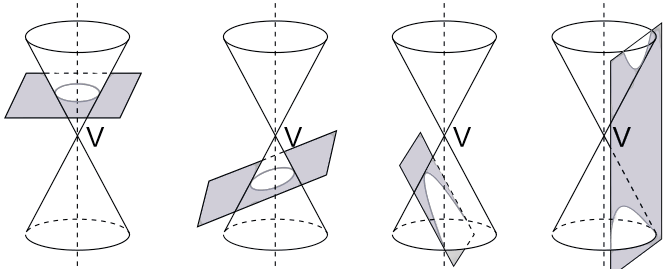
\includegraphics[width=0.5\linewidth]{images/conics.png}
\end{figure}
\begin{definition}[\textit{Conic}]
    A point $\mathbf{x}$ is considered to be on a conic $\mathbf{C}$ if it satisfies a homogeneous quadratic equation of the form:
    \[\mathbf{x}^TC\mathbf{x}=0\]
    Where $\mathbf{C}$ is a symmetric matrix is a symmetric matrix, which is a convention.
\end{definition}
Conics are curves described by second-degree equations in the plane. 
In Euclidean coordinates, a conic can be expressed as:
\[aX^2+bXY+cY^2+dX+eY+f=0\]
In homogeneous coordinates, it becomes:
\[ax^2+bxy+cy^2+dxw+eyw+fw^2=0\]
Alternatively, it can be represented in matrix form as:
\[\mathbf{x}^T \begin{bmatrix} a & b/2 & d/2 \\ b/2 & c & e/2 \\ d/2 & e/2 & f \end{bmatrix} \mathbf{x}=0\]
Conics have five degrees of freedom, which means that five points are required to uniquely define a conic.
\begin{example}
    A circle can be expressed in Cartesian coordinates as:
    \[(x-x_0)^2+(y-y_0)^2-r^2=0\]
    In homogeneous coordinates, it is represented as:
    \[\begin{bmatrix} x & y & w \end{bmatrix} \begin{bmatrix} 1 & 0 & -x_0 \\ 0 & 1 & -y_0 \\ -x_0 & -y_0 & x_0^2+y_0^2-r^2 \end{bmatrix} \begin{bmatrix} x \\ y \\ w \end{bmatrix} = 0\]
\end{example}

When you have a quadratic equation representing a conic and a linear equation for a line, their intersection results in a second-degree equation for the point $\mathbf{x}$. 
Consequently, there will always be two intersection points between a line and a conic. 
These intersection points can fall into one of the following categories:
\begin{itemize}
    \item \textit{Real and distinct}: this occurs when the line and conic intersect at two separate, real points.
    \item \textit{Real and coincident}: in this case, the line and conic intersect at a single real point, but it is a repeated or double root of the equation.
    \item \textit{Complex and distinct}: the intersection points are two complex conjugate points.
    \item \textit{Complex and coincident}: the line and conic intersect at a single complex point, and it is a repeated or double root.
\end{itemize}
This behavior is due to the fundamental theorem of algebra, which guarantees that a second-degree equation will have exactly two solutions when considering complex numbers.
\begin{figure}[H]
    \centering
    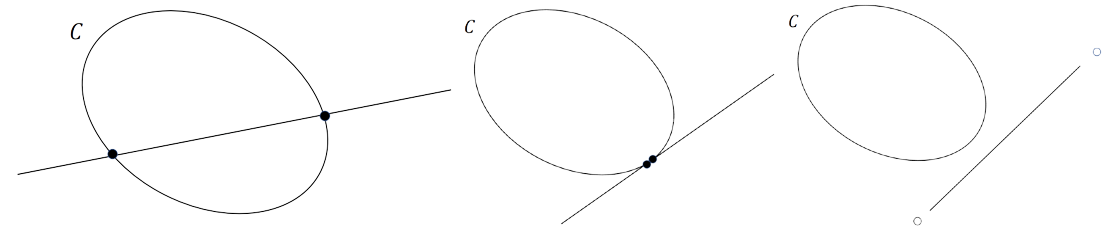
\includegraphics[width=0.75\linewidth]{images/intersection.png}
    \caption{Intersection with two real roots, two coincident roots and two imaginary roots}
\end{figure}
The intersection between the line at infinity and a conic results in the following scenarios:
\begin{itemize}
    \item \textit{Parabola}: when there are two coincident solutions, indicating the point at infinity along the axis.
    \item \textit{Ellipse}: when there are two complex-conjugate solutions, meaning there are no real solutions.
    \item \textit{Hyperbola}: when there are two real and distinct solutions, representing lines that serve as the asymptotes.
\end{itemize}

\subsection{Circular points}
\begin{example}
    When we intersect a circumference and the line at infinity, we obtain the following system:
    \[\begin{cases}
        x^2-2x_0w+x_0^2w^2+y^2-2y_0w+y_0^2w^2-r^2w^2=0 \\
        w=0
    \end{cases}\]
    This system simplifies to: 
    \[x^2+y^2=0\]
    It's evident that the parameters of the circumference (center and radius) have disappeared from the equation. 
    Consequently, the two intersection points are the same for all circumferences.    
\end{example}
\begin{definition}[\textit{Circular points}]
    The two intersection points remain the same for all circumferences when intersected with the line at infinity are referred to as the circular points.
    These points are defined as:
    \[\mathbf{I}=\begin{bmatrix} 1 \\ i \\ 0 \end{bmatrix} \qquad \mathbf{J}=\begin{bmatrix} 1 \\ -i \\ 0 \end{bmatrix}\]
\end{definition}

\subsection{Polar line}
\begin{definition}[\textit{Polar line}]
    Given a point $\mathbf{y}$ and a conic $\mathbf{C}$ in the plane, the line $\mathbf{l}=\mathbf{Cy}$ is called the polar line of point $\mathbf{y}$ with respect to the conic $\mathbf{C}$. 
\end{definition}
\begin{figure}[H]
    \centering
    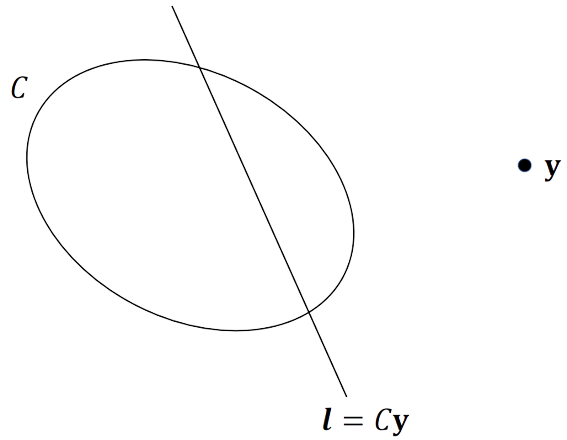
\includegraphics[width=0.3\linewidth]{images/polar.png}
    \caption{Example of polar line}
\end{figure}

\subsection{Harmonic tuples}
\begin{definition}[\textit{Harmonic tuple}]
    A 4-tuple of co-linear points $\mathbf{a}, \mathbf{b}, \mathbf{c}, \mathbf{d}$, whose cross ratio is = -1, is referred to as a harmonic tuple. 
\end{definition}
This specific value of the cross ratio is also shared by other 4-tuples of co-linear points. 
A notable example is:
\[\left( \mathbf{y},\mathbf{z},\text{mid point}(\mathbf{y},\mathbf{z}),P(\text{at the infinity}) \right)\]
Furthermore, if $(\mathbf{a}, \mathbf{b}, \mathbf{c}, \mathbf{d})$ is a harmonic 4-tuple, then $(\mathbf{c}, \mathbf{d}, \mathbf{a}, \mathbf{b})$ is also harmonic. 
\begin{definition}[\textit{Conjugate}]
    In a harmonic tuple $(\mathbf{a}, \mathbf{b}, \mathbf{c}, \mathbf{d})$, points $\mathbf{a}$ and $\mathbf{b}$ are said to be conjugate of each other concerning points $\mathbf{c}$ and $\mathbf{d}$.
\end{definition}
Since the cross ratio of a harmonic tuple is negative, it follows that two conjugate points, $\mathbf{a}$ and $\mathbf{b}$, concerning $\mathbf{c}$ and $\mathbf{d}$, are positioned in such a way that one is located within the segment ($\mathbf{c}, \mathbf{d}$), while the other is situated outside this segment.

\subsection{Polar line and harmonic tuples}
Take any point $\mathbf{z}$ on the polar line $\mathbf{l}=\mathbf{Cy}$ and then consider the line passing through points $\mathbf{y}$ and $\mathbf{z}$. 
Let's denote by $\mathbf{x}_1$ and $\mathbf{ax}_2$ the points at which this line intersects the conic.    
\begin{figure}[H]
    \centering
    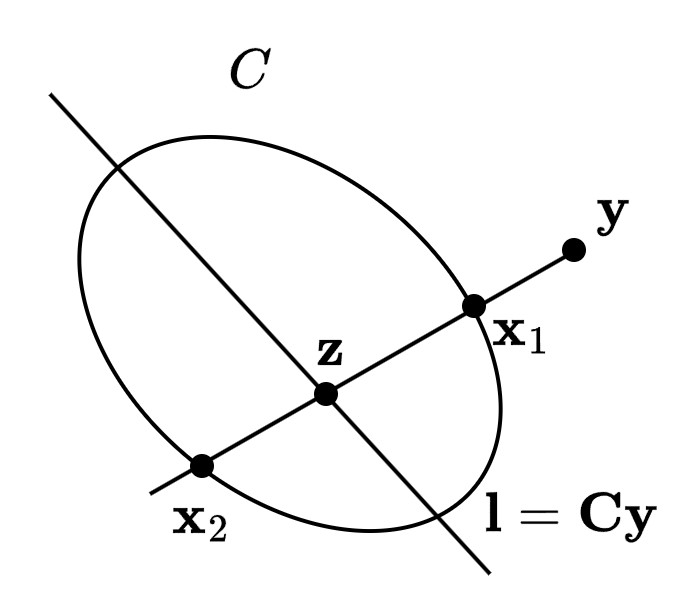
\includegraphics[width=0.25\linewidth]{images/polarharmonic.png}
\end{figure}
\begin{theorem}
    Let $\mathbf{x}_1$ and $\mathbf{x}_2$ represent the points at which the line passing through $\mathbf{y}$ and $\mathbf{z}$ intersects the conic $\mathbf{C}$. 
    In this case, $\mathbf{y}$ and $\mathbf{z}$ are conjugate with respect to $\mathbf{x}_1$ and $\mathbf{x}_2$.     
\end{theorem}
The polar line $\mathbf{l}=\mathbf{Cy}$ represents the set of points that are conjugate to $\mathbf{y}$ with respect to the conic $\mathbf{C}$.
More precisely, it includes points that are conjugate with respect to the intersection points of $\mathbf{C}$ with any line passing through $\mathbf{y}$.

\subsection{Polar line and tangency points}
As the line through $\mathbf{y}$ approaches tangency with the conic $\mathbf{C}$, the points $\mathbf{x}_1$ and $\mathbf{x}_2$ coincide with the points of tangency to $\mathbf{C}$. 
Consequently, the conjugate point $\mathbf{z}$, which remains within the interval ($\mathbf{x}_1,\mathbf{x}_2$), also coincides with the tangency point. 
This applies to any line that is tangent to $\mathbf{C}$ from the point $\mathbf{y}$.
Therefore, we have established that the polar line $\mathbf{l}=\mathbf{Cy}$ passes through the points of tangency from $\mathbf{y}$ to the conic $\mathbf{C}$. 

This leads us to the conclusion that if a point $\mathbf{z}$ lies on the conic $\mathbf{C}$, then point $\mathbf{y}$ is one of its conjugates with respect to the same conic. 
The tangent line $\mathbf{lz}$ to the conic $\mathbf{C}$ passing through point $z\mathbf{z}$ is the set of points that are conjugate to $\mathbf{z}$. 
Therefore, we can assert that $\mathbf{lz}$ is the polar line of $\mathbf{z}$ with respect to conic $\mathbf{C}$.
\begin{figure}[H]
    \centering
    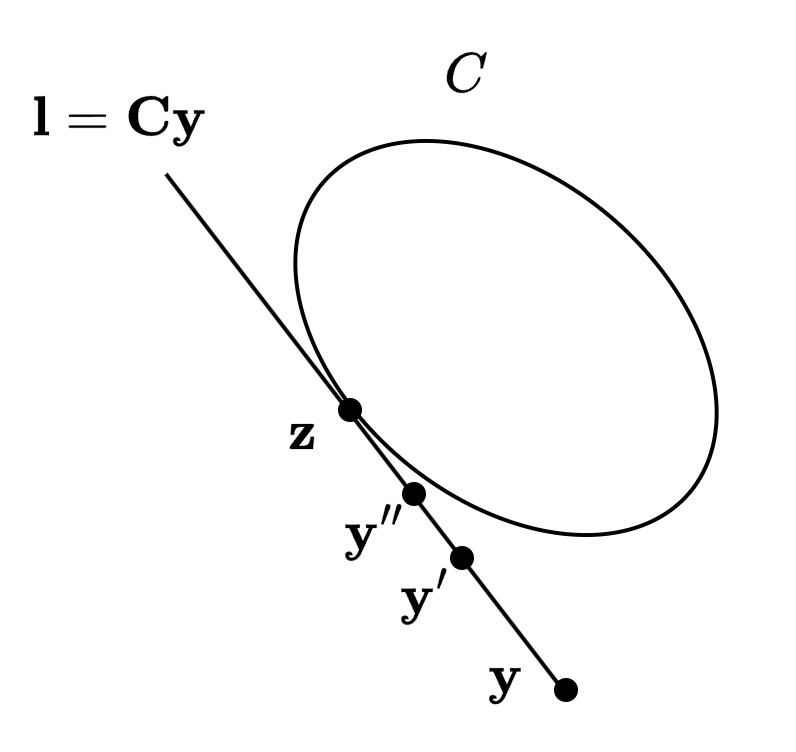
\includegraphics[width=0.4\linewidth]{images/tangentpolar.png}
\end{figure}
In the accompanying illustration, you can observe that the polar line $\mathbf{lz} = \mathbf{Cz}$ for a point $\mathbf{z}$ situated on the conic $\mathbf{C}$ corresponds to the tangent line to the conic $\mathbf{C}$ at the point $\mathbf{z}$.
\begin{example}
    Consider a circumference with radius $r$ centered in the origin of the plane and the point $\mathbf{y}={\begin{bmatrix} x & 0 & 1 \end{bmatrix}}^T$. 
    The equation of the polar line is given by:
    \[\mathbf{l}=\mathbf{Cy}=\begin{bmatrix} 1 & 0 & 0 \\ 0 & 1 & 0 \\ 0 & 0 & -r^2 \end{bmatrix} \begin{bmatrix} \mathbf{x} \\ 0 \\ 1 \end{bmatrix} = \begin{bmatrix} \mathbf{x} \\ 0 \\ -r^2 \end{bmatrix}\]
    Therefore, the Cartesian equation of the polar line becomes: 
    \[\mathbf{x} x-r^2 = 0 \rightarrow x=\dfrac{r^2}{\mathbf{x}}\]
    This equation describes a vertical line.
\end{example}

From the previous example, we can conclude that the polar of a point $\mathbf{p}$ with respect to a circle is a line that is perpendicular to the line segment connecting the center of the circle to point $\mathbf{p}$. 
\begin{example}
    Consider a circumference with radius $r$ centered in the origin of the plane and the point $\mathbf{y}={\begin{bmatrix} x & 0 & 0 \end{bmatrix}}^T$.
    The equation of the polar line is given by:
    \[\mathbf{l}=\mathbf{Cy} = \begin{bmatrix} 1 & 0 & 0 \\ 0 & 1 & 0 \\ 0 & 0 & -r^2 \end{bmatrix} \begin{bmatrix} \mathbf{x} \\ 0 \\ 0 \end{bmatrix} =  \begin{bmatrix} \mathbf{x} \\ 0 \\ 0 \end{bmatrix}\]
    Therefore, the Cartesian equation of the polar line becomes: 
    \[\mathbf{x} x=0 \rightarrow \mathbf{x}=0\]
    This equation describes the diameter of the circumference perpendicular at the direction of the point $\mathbf{y}$. 
\end{example}
Tangent lines emerging from a point at infinity are always parallel. 
Consequently, the points of tangency lie along a diameter that is perpendicular to the direction of these parallel tangents.    
\begin{figure}[H]
    \centering
    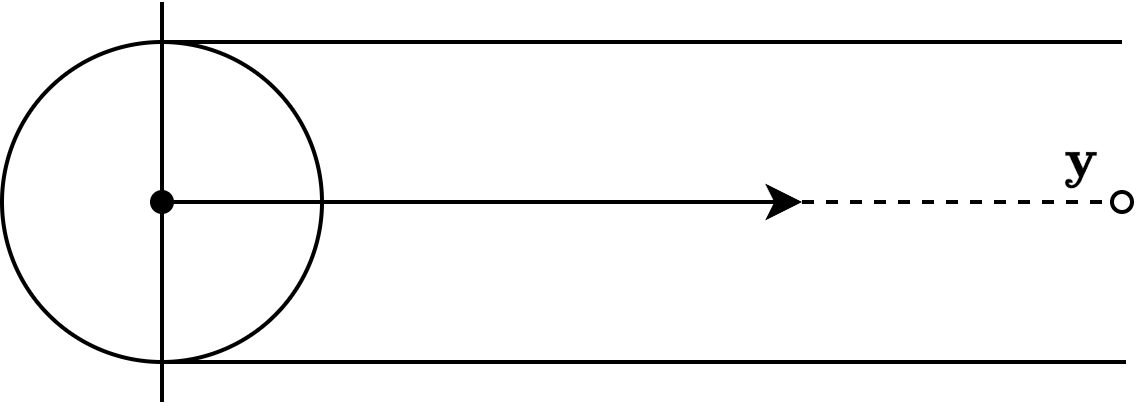
\includegraphics[width=0.5\linewidth]{images/parallel.png}
\end{figure}
\begin{example}
    Consider a circumference with radius $r$ centered in the origin of the plane and the point $\mathbf{y}={\begin{bmatrix} x & 0 & 0 \end{bmatrix}}^T$.
    The equation of the polar line is given by:
    \[\mathbf{l}=\mathbf{Cy}=\begin{bmatrix} 1 & 0 & 0 \\ 0 & 1 & 0 \\ 0 & 0 & -r^2 \end{bmatrix}\begin{bmatrix} 0 \\ 0 \\ 1 \end{bmatrix} = \begin{bmatrix} 0 \\ 0 \\ -r^2 \end{bmatrix}\]
    Therefore, the Cartesian equation of the polar line becomes: 
    \[-r^2w=0 \rightarrow \mathbf{x}=0\]
    This equation describes the line at the infinity. 
\end{example}
Here are the general properties of the polar lines.
\begin{property}
    The polar line of any point at infinity is a diameter.
\end{property}
\begin{property}
    Any diameter goes through the center of the circle.
\end{property}
\begin{property}
    The center is conjugate to every point at infinity.
\end{property}
\begin{property}
    All points at infinity are conjugate to the center.
\end{property}
\begin{property}
    The polar of the center is the line that includes all the points at infinity.
\end{property}
\begin{property}
    The polar line of the center is the line at infinity.
\end{property}

\subsection{Degenerate conics}
\begin{definition}[\textit{Non-degerate conic}]
    A non-degenerate conic is a conic where the matrix $\mathbf{C}$ is non-singular, indicating that: 
    \[\textnormal{rank}(\mathbf{C})=3\]
\end{definition}
\begin{definition}[\textit{Degerate conic}]
    Conversely, a degenerate conic is a conic  for which the matrix $\mathbf{C}$ is singular, characterized by: 
    \[\textnormal{rank}(\mathbf{C}) < 3\]
\end{definition}
There are two distinct scenarios to consider:
\begin{itemize}
    \item When $\textnormal{rank}(\mathbf{C}) = 2$, any symmetric $3 \times 3$ matrix $\mathbf{C}$ can be expressed as:
        \[\mathbf{C}=\mathbf{lm}^T+\mathbf{ml}^T\]
        Here, $\mathbf{l}$ and $\mathbf{m}$ are column vectors. 
        The conic corresponds to the set of points $\mathbf{x}$  that satisfy $\mathbf{x}^T\mathbf{Cx}=0$.
        This equation is met when either $\mathbf{x}^T\mathbf{l}=0$ or $\mathbf{m}^T\mathbf{x}=0$. 
        Consequently, $\mathbf{x}$ lies on the union of lines represented by $\mathbf{l}$ and $\mathbf{m}$
        \begin{figure}[H]
            \centering
            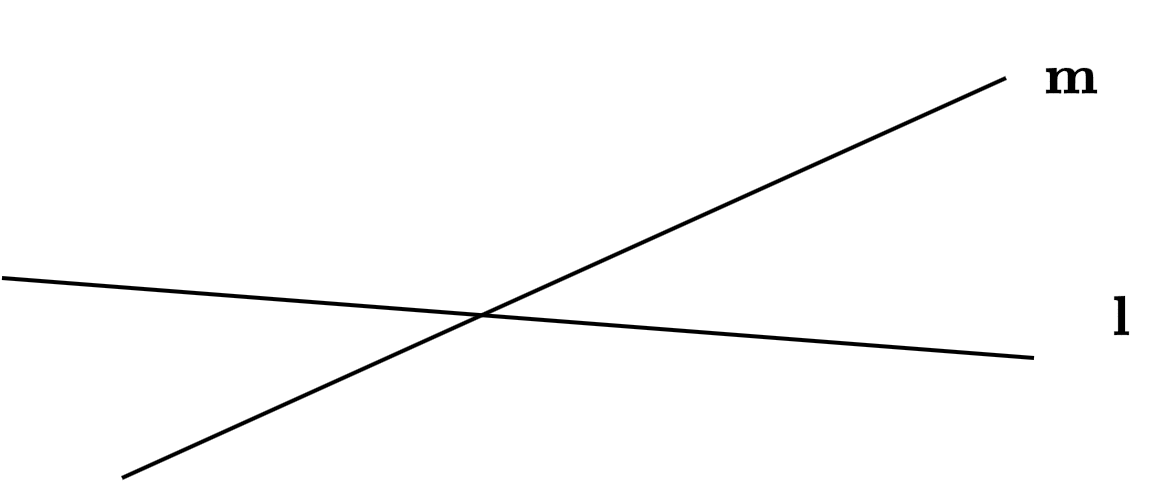
\includegraphics[width=0.25\linewidth]{images/inters.png}
        \end{figure}
    \item When $\textnormal{rank}(\mathbf{C}) = 1$, a symmetric $3 \times 3$ matrix $\mathbf{C}$ can be expressed as:
        \[\mathbf{C}=\mathbf{ll}^T\]
        In this case, $\mathbf{l}$ is a column vector. 
        The conic consists of the points $\mathbf{x}$ that satisfy $\mathbf{x}^T\mathbf{Cx}=0$.
        This equation holds  when $\mathbf{x}^T\mathbf{l}=0$ is met (twice). 
        Thus, $\mathbf{x}$ is on the repeated line represented by $\mathbf{l}$.
        \begin{figure}[H]
            \centering
            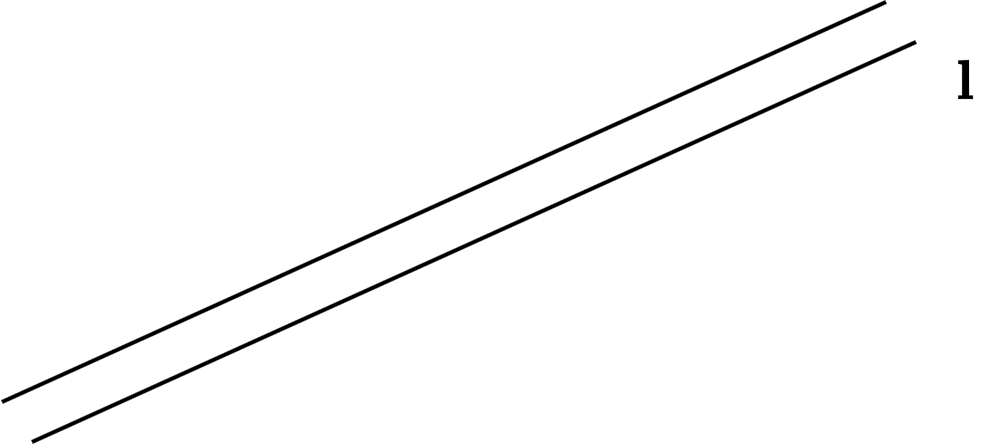
\includegraphics[width=0.25\linewidth]{images/rep.png}
        \end{figure}
\end{itemize}